\documentclass[12pt]{article}

\usepackage{minted}
\usemintedstyle{emacs}
\usepackage{cite}
\usepackage[pdftex]{graphicx}
\usepackage{amsmath}
\usepackage[table,x11names]{xcolor}

\usepackage[margin=1.25in]{geometry}
\usepackage[doublespacing]{setspace}

%opening
\title{LIN5111 Project 5\\Sentiment Analysis of Facebook Posts}
\author{Thuong-Hai Pham}

\begin{document}

\maketitle

\section{Introduction}
Alongside with the expansion of social networks, online marketing and, in general, digital revolution, sentiment analysis plays an important role for companies, governments and any organisation to gain actionable insights from their customers, citizen and members.

In brief, sentiment analysis can be described simply by a task which tells whether the given piece of text/speech is positive, negative or neutral although the expected output may be more complex with more fine-grained classes or even continuous real value of intensity. However, it is important to note that there is some differences between sentiment analysis and emotion analysis in which we try to predict emotional feelings (e.g. sadness, anger...)

In the scope of this report about sentiment analysis, we are going to discuss what features of text dataset can be taken into our predictive model, the possible classifiers and regressors in section \ref{background}. Consequently, the preprocessing phase of our experiment data is introduced in section \ref{data} which then being continued by our methodology and experimental results in detail with section \ref{method} and \ref{results}, respectively. Afterwards, conclusion and further improvements are presented in section \ref{conclusion}.

\section{Background} \label{background}

\subsection{Features}

In sentiment analysis, these features can be taken into our consideration:
\begin{itemize}
	\item \textbf{Bag of Words} is very straightforward approach when all of the word counts (or presences, whether that word type exists or not) represent as features of the sentence. More advance, TF-IDF can be used to overcome high/low word frequencies problem in Bag of Words.

	\item \textbf{Sentiment lexicon}. In which we compute the sentiment value of the whole sentence by each individual tokens/phrases built up the sentence. These tokens/phrases values are defined in a manual/semi-manual constructed lexicon. The value can be either in form of positive/negative label or intensity.

	\item \textbf{Negation}. When using \textbf{sentiment lexicon}, one problem may emerge is the negation of phrases. For instance, ``good" has the positive value, yet ``not good" should hold a negative one. One may solve this problem by negating value of all words occurring between a negator (not, never, no...) and a punctuation. Nevertheless, negated words, in case of real value sentiment lexicon, need to be specified exact sentiment value, which is not trivial by inverting its counterpart number (0.7 to -0.7) as ``not good" does not mean ``bad". Other approach is to make use of sentiment lexicon with negator-head phrases support.
	
	\item \textbf{Capitalisation} is very intuitive feature by having that writer, especially social media users, tend to use all-capitalised-character words to show strong emotions.
	
	\item \textbf{Elongated words}, besides \textbf{capitalisation}, are also commonly used to convey strong emotion, such as ``Hoooorayyyy".
	
	\item \textbf{Emoticons} are very straightforward and distinct way for writer to show their feelings by indicating that he/she is smiling, crying...

	\item \textbf{Symbols} or \textbf{punctuations} can also play as a hint to writer's feelings. A series of exclamation marks may imply a degree of high intensity. While a group of arbitrary symbols as ``@\%\#\^\$" may show negative feeling toward mentioned subject.
	
	\item With recent advance in neural network for distributional semantics, \textbf{semantic representation} may serve as promising unsupervised features by determining sentence meaning through vector representation. This representation can be used to train our model easily in sentiment analysis task. These \textbf{semantic representation} may be learnt by distributional semantics method or recent neural network approach such as word2vec \cite{mikolov2013distributed} or more sentence-focused doc2vec \cite{le2014distributed}.
\end{itemize}

\subsection{Regression or Classification}

The sentiment analysis task can be classified as regression or classification problem depends on the output we would like to achieve.

\subsubsection{Classification}
As a classification problem, our task is to determine whether the given text is positive or negative (coarse-grained classification). The output label may be more fine-grained by divided into more classes: extremely negative, negative, neutral, positive, extremely positive.

For the classification problem, the common and basic approach is \textbf{Naive Bayes}, which holds the assumption of in-dependency between features. More advance, \textbf{Nearest Neighbour}, \textbf{Decision Tree} or \textbf{Random Forest}, a ensemble of decision trees that is very popular among industrial data science task, can be used. To achieve more complex model, we can take into our consideration \textbf{Support Vector Machine (SVM)} or Neural Net. SVM uses a kernel to transform our data into a higher dimensional space, then find the linear cut to separate the data. While \textbf{Neural Net} simulates complex function to attain our true labels by combining weighted from many neurons on different layers of the network. Please be noted that the latter approaches may not work well with Bag-of-words features due to its sparseness.

\subsubsection{Regression}

When coming to regression model, we prefer to attain continuous real values as the output instead of discrete labels. In this manner, \textbf{Linear Regression} comes first with its simplicity by solving, mathematically, the problem in form:
\[\min_w{||Xw-y||_2}^2\]
in which $X$ and $y$ are our features matrix and label vector, respectively, $w$ is the set of weights we want to learn from training data, the norm used in this formula is $L^2$ norm (or Euclidean norm).

Nevertheless, applying Linear Regression on a set which consists of some linear-dependent features may cause the model to be over-fitted (works well on training data but worse on testing data by remembering the data instead of generalising them) . Hence, \textbf{Ridge} (linear regression with $L^2$ regulariser) is introduced to solve this problem by imposing a penalty on the size of the coefficients in the model through attempting to minimise a penalised residual sum of squares as,
\[\min_w{||Xw-y||_2}^2+\alpha{||w||_2}^2 \]
in which $\alpha$ is the complexity parameter, i.e. the larger $\alpha$ is, the more shrinkage we would like to apply so our model coefficients become more robust to collinearity.

Being different from Ridge regression which only reduces the coefficients, \textbf{Lasso} (linear regression with $L^1$ regulariser) eliminates coefficients that are linear dependent on the others by introducing $L^1$ norm of the parameter vector $||w||_1$ in objective function:
\[\min_w\frac{1}{2n_{samples}}{||Xw-y||_2}^2+\alpha||w||_1\]

Besides linear regression family, there are also counterparts of the more complex regression methods introduced in the previous section can be used as or regressor such as \textbf{Random Forest Regressor}, \textbf{Support Vector Machine Regressor} (SVR) or \textbf{Stochastic Gradient Descent} (SGD) which suit the problem of large number of samples, yet not sparse.

\section{Data} \label{data}

\subsection{Training \& testing data} \label{main_data}

Our main data, 2896 Facebook status updates hand-labelled with valence and arousal, is acquired from myPersonality Project\footnote{http://mypersonality.org/wiki/doku.php?id=start}
\begin{table}[H]
	\centering
	\begin{tabular}{| c | l | c | c | c | c |}
		\hline
		& \textbf{text} & \textbf{val1} & \textbf{val2} & \textbf{aro1} & \textbf{aro2}\\
		\hline
		0 & We'll be off and running to a lil' place calle... & 9 & 9 & 8 & 8\\
		\hline
		1 & I really wana move soon! & 4 & 5 & 5 & 7\\
		\hline
		2 & thinking at charity cup & 5 & 5 & 1 & 1\\
		\hline
		3 & thinks that for girls, boys are easily found. ... & 4 & 3 & 6 & 7\\
		\hline
		4 & Our Wedding Anniversary tonight... & 7 & 7 & 4 & 5\\
		\hline
	\end{tabular}
	\caption{Top lines of the acquired data}
	\label{tb:data_first_lines}
\end{table}

In table \ref{tb:data_first_lines} above, ``text" column represents original Facebook status updates from users\cite{preotiuc2016modelling}, which were already anonymised by replacing people names, urls, addresses and phone numbers with $\langle$PERSON$\rangle$, $\langle$URL$\rangle$, $\langle$ADDRESS$\rangle$, $\langle$PHONE$\rangle$, respectively. Val1, val2 are valence (from 1 to 9) assigned by two distinct judges. While aro1, aro2 are arousal (from 1 to 9) assigned in the same way.

\subsection{Sentiment lexicon} \label{sentiment_lexicon}
In addition to our main data, we need a sentiment lexicon to perform feature extraction of sentiment value from tokens/phrases. For instance, to check whether ``happy" is positive or negative, and how positive/negative it is.

There are some lexicon that suite our need such as General Inquirer \cite{stone1966general}, MPQA \cite{wiebempqa}, Hu and Liu lexicon \cite{hu2004mining}. However, we choose Sentiment Composition Lexicon of Negators, Modals, and Adverbs (SCL-NMA) \cite{SCL-NMA} as it provides us lexicon entry for phrases starting with negators and supports intensity instead of only positive/negative labels.

\subsection{Data preprocessing}

However, our data is not flawless. There are some missing cells in the table, so the most convenient way is to drop those missing (or N/A) values from the table, which results in 2894 entries left. These 2894 entries are then divided \textbf{training set of 2315 entries} and \textbf{test set of 579 entries}, the ratio of 80:20.

\subsubsection{Target normalisation}
In this data preprocessing process, we also average the two judges' scores and normalise our valence and arousal value to the range of (0..1) for unity in further comparisons.
\begin{table}[H]
	\centering
	\begin{tabular}{| l | l | l | l | l | l | l |}
		\hline
		& \textbf{val1} & \textbf{val2} & \textbf{aro1} & \textbf{aro2} & \textbf{val} & \textbf{aro}\\
		\hline
		\textbf{count} & 2894 & 2894 & 2894 & 2894 & 2894 & 2894\\
		\hline
		\textbf{mean} & 5.274015 & 5.250173 & 3.363856 & 3.343124 & 0.532762 & 0.294186\\
		\hline
		\textbf{std} & 1.042098 & 1.485600 & 1.958775 & 2.183769 & 0.148835 & 0.247551\\
		\hline
		\textbf{min} & 2.000000 & 1.000000 & 1.000000 & 1.000000 & 0.062500 & 0.000000\\
		\hline
		\textbf{25\%} & 5.000000 & 5.000000 & 2.000000 & 1.000000 & 0.437500 & 0.062500\\
		\hline
		\textbf{50\%} & 5.000000 & 5.000000 & 3.000000 & 3.000000 & 0.500000 & 0.187500\\
		\hline
		\textbf{75\%} & 6.000000 & 6.000000 & 5.000000 & 5.000000 & 0.625000 & 0.500000\\
		\hline
		\textbf{max} & 9.000000 & 9.000000 & 9.000000 & 9.000000 & 1.000000 & 1.000000\\
		\hline
	\end{tabular}
	\caption{Valence and Arousal values}
	\label{tb:val_aro_processed}
\end{table}
The latter phases of our methods then only use the val and aro columns, which are our averaged values.

\subsubsection{Contraction} \label{contraction}

In addition, we also need to deal with contractions because these may cause mismatching during our feature extraction from sentiment lexicon. For example, string matching of ``would be bad" and ``'d be bad" may return False even though they represent the same meaning. Hence, contractions are processed during this phases not on the text data but the sentiment lexicon itself. The reason is to recover expansion from text data contraction may lead to ambiguity, such as ``'d" can represent ``had" or ``would". While contracting existing phrases are more straightforward.

\begin{listing}[H]
	\begin{minted}{python}
contractions_1 = {"would ": "'d ", "have ": "'ve ", "will ": "'ll ",
		"had ": "'d "}
contractions_2 = {"would have ": "would've ", "would have ": "'d've ",
		"will not ": "won't ", "was not ": "wasn't ",
		"did not ": "didn't ", "could not ": "couldn't ",
		"does not ": "doesn't ", "do not ": "don't ",
		"would not ": "wouldn't ", "can not ": "cannot ",
		"cannot ": "can't ", "should not ": "shouldn't "}
	\end{minted}
	\caption{Contractions rule for generating new items in sentiment lexicon}
	\label{lst:contractions}
\end{listing}

Listing \ref{lst:contractions} shows list of rules we use to generate new entries in our sentiment lexicon by contraction. Please note that these rules do not cover all contractions in English language but small amount of hand-picked rules to cover our sentiment lexicon. Mostly, these contractions rules are related to negation and degree. Afterwards, we get \textbf{4092} entries in our final lexicon from 3214 original entries.

\section{Method} \label{method}

In fact, sentiment analysis as a classification tasks is widely explored albeit Bag-of-words and Naive Bayes can achieve pretty high accuracy. In addition, the data we use provides us with continuous real data for valence and arousal, so we consider our task as \textbf{regression problem} instead.

\subsection{Baseline algorithm}
For baseline algorithm, we use the Bag-of-words as our features, then train Linear Regression for our regressor with $L^2$-norm regularisation (Ridge) \cite{preotiuc2016modelling}.

\subsection{Features}
\subsubsection{Bag of Words}
To extract this feature, we use class ``CountVectorizer" of scikit-learn\footnote{http://scikit-learn.org/stable/} library with minimum occurrence (min\_df) of 3. We also try a more advance version with TF-IDF\footnote{Term Frequency and Inverse Document Frequency}, provided in the same library.

\subsubsection{Sentiment lexicon (lex)}
Sentiment lexicon feature in our model is represented by a real number, which is sum of all sentiment values from the words/phrases within the sentence. These values are determined by string matching and sentiment value from our sentiment lexicon described in section \ref{sentiment_lexicon}.

\subsubsection{Negation}
The problem of negation in our case is solved by phrases with negators in section \ref{sentiment_lexicon} and preprocessed with contraction as described in section \ref{contraction}.

\subsubsection{Capitalisation (char\_cap, full\_cap)}
For capitalisation, we are interested in all-character-capitalised words (full\_cap), which seems to show the writer's strong voice. In addition, we also count the total number of capital letters within the sentence (char\_cap). In both cases, we do not count the place holder for anonymised data: $\langle$PERSON$\rangle$, $\langle$URL$\rangle$, $\langle$ADDRESS$\rangle$, $\langle$PHONE$\rangle$ as described in section \ref{main_data}.

\subsubsection{Emoticons (emo)}
To attain emoticons feature, we use the following regular expression to extract emoticons from text
\mint{python}{"([;:=][-\"']?[\*P)(\]><]+|[\*P)(\]<>]+[-\"']?[;:=]|lol|<3)"}

Then, we consider these emoticons to be word by counting their occurrences. Listing \ref{lst:emoticons_feature} below gives us examples of two sentences in the training set and test set, respectively, with their emoticon feature. The dimension of this feature (16) is also the number of distinct emoticon types in our dataset.

\begin{listing}[H]
	\begin{minted}{text}
id   text     val     aro
1167  ":'("  0.1875  0.1875
0   1   2   3   4   5   6   7   8   9   10  11  12  13  14  15
0   0   1   0   0   0   0   0   0   0   0   0   0   0   0   0
id	text    				val   aro
1758  "So Far We still have school tomorrow :'("  0.375  0.25
0   1   2   3   4   5   6   7   8   9   10  11  12  13  14  15
0   0   1   0   0   0   0   0   0   0   0   0   0   0   0   0
	\end{minted}
	\caption{Samples of emoticon feature}
	\label{lst:emoticons_feature}
\end{listing}

\subsubsection{Elongated words (elong\_w)}
Elongated words are identified by a simple rule: any word that ends with 3 repeated letters are considered to be elongated words.

\subsubsection{Punctuations (punct\_ex, punct\_qt)}
In punctuation case, we separate two types and count occurrence of each type. The first type is exclamation mark (punct\_ex) ``!" which may denote high intensity in writer's feeling. The second type is any symbol in the set ``\%@\#*\&?\^" (punct\_qt), which usually used to inform inexpressible negative emotion.

\subsubsection{Semantic representation (doc2vec)}
To attain semantic representation of our sentences, we use doc2vec class from Gensim\footnote{https://radimrehurek.com/gensim/models/doc2vec.html} library. The reason why we employ doc2vec instead of word2vec is that our raw data unit to extract feature is sentence. While using word2vec requires a further step to combine the words representation into one.

Instead of running cross validation, we apply the hyper-parameters set suggested by the author which can reproduce the paper experiment at its best:
\begin{minted}{python}
dm=0, dbow_words=1, size=100, window=10, hs=0, negative=5,
 sample=1e-4, iter=20, min_count=1, workers=cores
\end{minted}

Listing \ref{lst:number_feature} below shows us some samples after features extraction phase, excluding semantic representation and emoticons.

\begin{listing}[H]
	\begin{minted}{text}
                                             text  lex  full_cap
                  internet is jackkked . love you  0.917       0
jus chillin i came in second in da 400 and thi... -0.006       0
                 ... And boom goes the dynamite .  0.000       0
i wish there was not any snow outside so i cou...  0.000       0
You can make what you don't understand mean an... -0.043       0

  char_cap  char_count  word_count  punct_ex  punct_qt  elong_w
         0          31           6         0         0        0
         0         127          28         0         0        0
         1          32           7         0         0        1
         0          54          12         0         0        0
         1          54          10         0         0        0
	\end{minted}
	\caption{Samples of features (without doc2vec \& emo)}
	\label{lst:number_feature}
\end{listing}

\subsection{Regression methods}
For this experiment, we consider running our model using Linear Regression and Linear Regression with $L^2$ normalisation (Ridge). 5-folds cross validation is also used to fine-tune the hyper-parameters (in this case is $\alpha$)

\subsection{Evaluation}
Beside two regressors chosen above, Mean Square Error (MSE) and coefficient of determination ($R^2$) are also selected to measure our model performance.
\[MSE=\frac{1}{n}\sum_{i=1}^{n}{(y_i-\hat{y}_i)^2}\]
in which, $y_i$ is the true value while $\hat{y}_i$ is our predicted value.
\[R^2=1-\frac{\sum_{i=1}^{n}{(y_i-\hat{y}_i)^2}}{\sum_{i=1}^{n}{(y_i-\bar{y})^2}}, \bar{y}=\sum_{i=1}^{n}y_i\]

While MSE is simple and intuitive, its interpretation depends heavily on the distribution of $y$. For example, MSE of 0.1 seems good to y in range (0, 100) but not (0, 1). On the other hand, $R^2$ is robust on this aspect. The maximum value of $R^2$ is 1, while our model correctly predicts all the outcome. While $R^2<0$ indicates that our model performance is worse than predicting a constant without looking into the input.

\section{Results} \label{results}


\subsection{Features comparison}
\begin{table}[H]
	\centering
	\begin{tabular}{| r | r | r | r | r |}
		\hline
		& \textbf{mse\_val} & \textbf{r2\_val} & \textbf{mse\_aro} & \textbf{r2\_aro}\\
		\hline
		\rowcolor{gray!50} \textbf{bow} & 0.015209 & 0.311061 & 0.058824 & -0.033189\\
		\textbf{all} & 0.014213 & \cellcolor{blue!25}0.356148 & 0.023093 & \cellcolor{blue!25}0.594395\\
		\textbf{drop\_char\_cap} & 0.014247 & 0.354633 & 0.023093 & 0.594388\\
		\textbf{drop\_char\_count} & 0.014246 & 0.354655 & 0.023076 & \cellcolor{blue!25}0.594684\\
		\textbf{drop\_doc2vec} & 0.014468 & 0.344619 & 0.023156 & 0.593280\\
		\textbf{drop\_elong\_w} & 0.014169 & \cellcolor{blue!25}0.358166 & 0.023340 & 0.590058\\
		\textbf{drop\_emo} & 0.016143 & \cellcolor{red!25}0.268714 & 0.023371 & 0.589511\\
		\textbf{drop\_full\_cap} & 0.014241 & 0.354909 & 0.023098 & 0.594311\\
		\textbf{drop\_lex} & 0.016183 & \cellcolor{red!25}0.266936 & 0.023085 & 0.594524\\
		\textbf{drop\_punct\_ex} & 0.015250 & 0.309185 & 0.053237 & \cellcolor{red!25}0.064944\\
		\textbf{drop\_punct\_qt} & 0.014416 & 0.346950 & 0.023222 & 0.592127\\
		\textbf{drop\_word\_count} & 0.014215 & \cellcolor{blue!25}0.356078 & 0.023077 & \cellcolor{blue!25}0.594666\\
		\hline
	\end{tabular}
	\caption{Features comparison}
	\label{tb:features_comp}
\end{table}

Table \ref{tb:features_comp} shows us the result of our attempt to compare between features\footnote{with Ridge as regressor}. Our baseline algorithm is in grey which arousal $R^2$ score is less than zero. Hence, the baseline algorithm performance on Arousal task is worse than a regressor outputs only constant value without analysing the input.

In the same table, light blue cells indicate features when dropped do not affect much on our final result. While dropping features with light red cells will significantly decline our performance.

Figure \ref{fig:features} highlights the declination in our model performance when leaving out one features. It is evident that emo and lex play important roles in our model, along with punct\_ex for Valence prediction task. While leaving out emo and lex, our model performs worse than the baseline algorithm. This can be explained by the fact that emoticons, as discussed above, are direct and obvious way for writer to express their emotion, while sentiment lexicon indicate clearly sentiment value of each words/phrases that build up our sentences.

On the other hand, in Arousal prediction task, puct\_ex is crucial for our model performance. With this proof, it can be said that writers/users tend to use exclamation mark to indicate their feeling raise more than any other linguistic features while writing.

\begin{figure}[H]
	\centering
	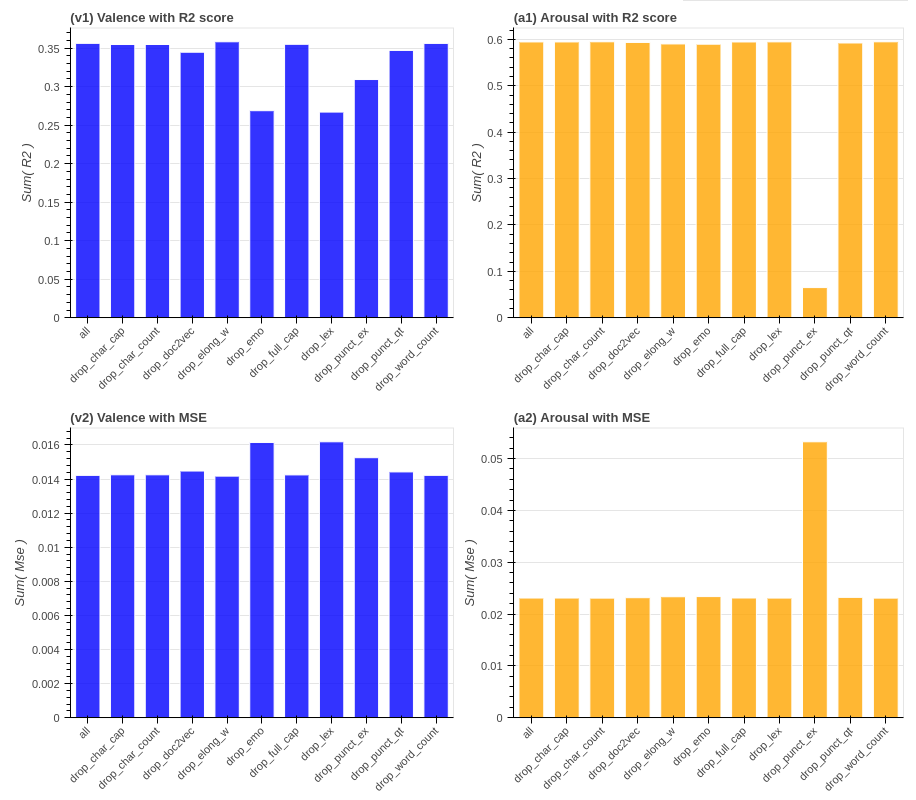
\includegraphics[width=\textwidth]{features}
	\caption{Features comparison}
	\label{fig:features}
\end{figure}

In addition, $R^2$ score (first row with (v1), (a1)) and MSE (second row with (v2), (a2)) show a high correlation between the two scores. 

\subsection{Regressor comparison}
In table \ref{tb:regr_comp}, Ridge demonstrates a better performance on both tasks by preventing over-fitting with $L^2$ normalisation.

\begin{table}[H]
	\centering
	\begin{tabular}{| r | r | r | r | r |}
		\hline
		& \textbf{mse\_val} & \textbf{r2\_val} & \textbf{mse\_aro} & \textbf{r2\_aro}\\
		\hline
		\textbf{Linear regression} & 0.016131 & 0.269272 & 0.024873 & 0.563122\\
		\textbf{Ridge} & 0.014213 & 0.356148 & 0.023093 & 0.594395\\
		\hline
	\end{tabular}
	\caption{Regressor comparison (on all features)}
	\label{tb:regr_comp}
\end{table}

\subsection{BoW variants}
In an attempt to try between BoW variants as our model features, unigram, combination of (1, 2, 3)-grams and TF-IDF have been tested with help of Ridge (linear regression with $L^2$ regularisation).

\begin{table}[H]
	\centering
	\begin{tabular}{| r | r | r | r | r |}
		\hline
		& \textbf{mse\_val} & \textbf{r2\_val} & \textbf{mse\_aro} & \textbf{r2\_aro}\\
		\hline
		\textbf{unigram} & 0.015209 & 0.311061 & 0.058824 & -0.033189\\
		\textbf{(1, 2, 3)-grams} & 0.015213 & 0.310844 & 0.059120 & -0.038393\\
		\textbf{TF-IDF} & 0.015218 & 0.310645 & 0.059120 & -0.038395\\
		\hline
	\end{tabular}
	\caption{Bag-of-words variants comparison}
	\label{tb:bow_comp}
\end{table}

It is obvious that there is not much different between all the variants. $R^2$ score for all of these features still far less than zero.

\section{Conclusion} \label{conclusion}

After analysing our results with the proposed features and regressors, our model clearly outperforms the simple Bag-of-words model in both tasks. It is clear that Bag-of-words feature does not help in Arousal task ($R^2 < 0$). More importantly, emoticons and sentiment lexicon prove their crucial roles for Valence prediction task. While exclamation mark is clearly the most significant feature for Arousal prediction task. These features can be explained by the manner writers/social media users use to express their feelings toward mentioned subjects.

We also attempt to use the semantic representation of sentence and paragraph through doc2vec library, which shows its acceptable effect in the tasks, but not significantly. This can be excused by the fact that we train the doc2vec model as an unsupervised meaning/feature learning task, which illustrated by diagram (b) Distributed Bag of Words in figure \ref{fig:doc2vec}.

\begin{figure}[t]
	\centering
	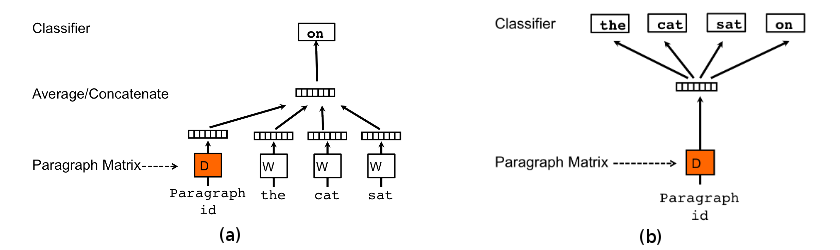
\includegraphics[width=\textwidth]{doc2vec}
	\caption{Framework for learning paragraph vector, (a) Distributed Memory, (b) Distributed Bag of Words}
	\label{fig:doc2vec}
\end{figure}

In future work, we can train this model by Distributed Memory network, in which the prediction task and loss function ($R^2$ or MSE) are integrated directly in the final layer of our network, as in diagram (a).

\bibliography{report}{}
\bibliographystyle{apalike}
\end{document}
